While the smart contracts represent the backbone of GETACAR, it is the frontend for customers and ride providers that enables the users to interact with the Platform. The developed prototype provides a fully designed frontend  for customers. The ride provider frontend is built as a service daemon called Virtual Vehicle that could be utilised by autonomous vehicles to interact with the platform and atomically interacts with the platform by posting bids on new rides and interacting with the ride contracts. 

\subsection{Customer Frontend Flow}
The customer frontend prototype is built using Angular \footnote{https://angular.io} and the web3 package \footnote{https://www.npmjs.com/package/web3} to interact with the Ethereum blockchain and crypto wallets. While the market-ready implementation of a decentralised ride-pooling platform would probably utilise native smartphone apps, the Angular web implementation allows for a fast, platform-independent development to showcase the most important features of the customer ride-pooling frontend. 

The customer frontend follows the three view design approach described in \ref{subsec:UserFrontend}, offering a booking view, an on-ride view and a settings view. 

The process of ordering a ride follows the customer flow seen in \ref{fig:RideBookingFlow} by opening the app and entering the destination and pickup location. The customer frontend provides a map that can preview the trip. Additionally, the frontend provides  a compass needle button as part of the pickup location input field. Pressing this button allows the customer to select their current location as their pickup location, shown in \ref{fig:MapScreen}.

\begin{figure}[H]
    \centering
    
    \begin{minipage}{0.45\linewidth}
        \centering
        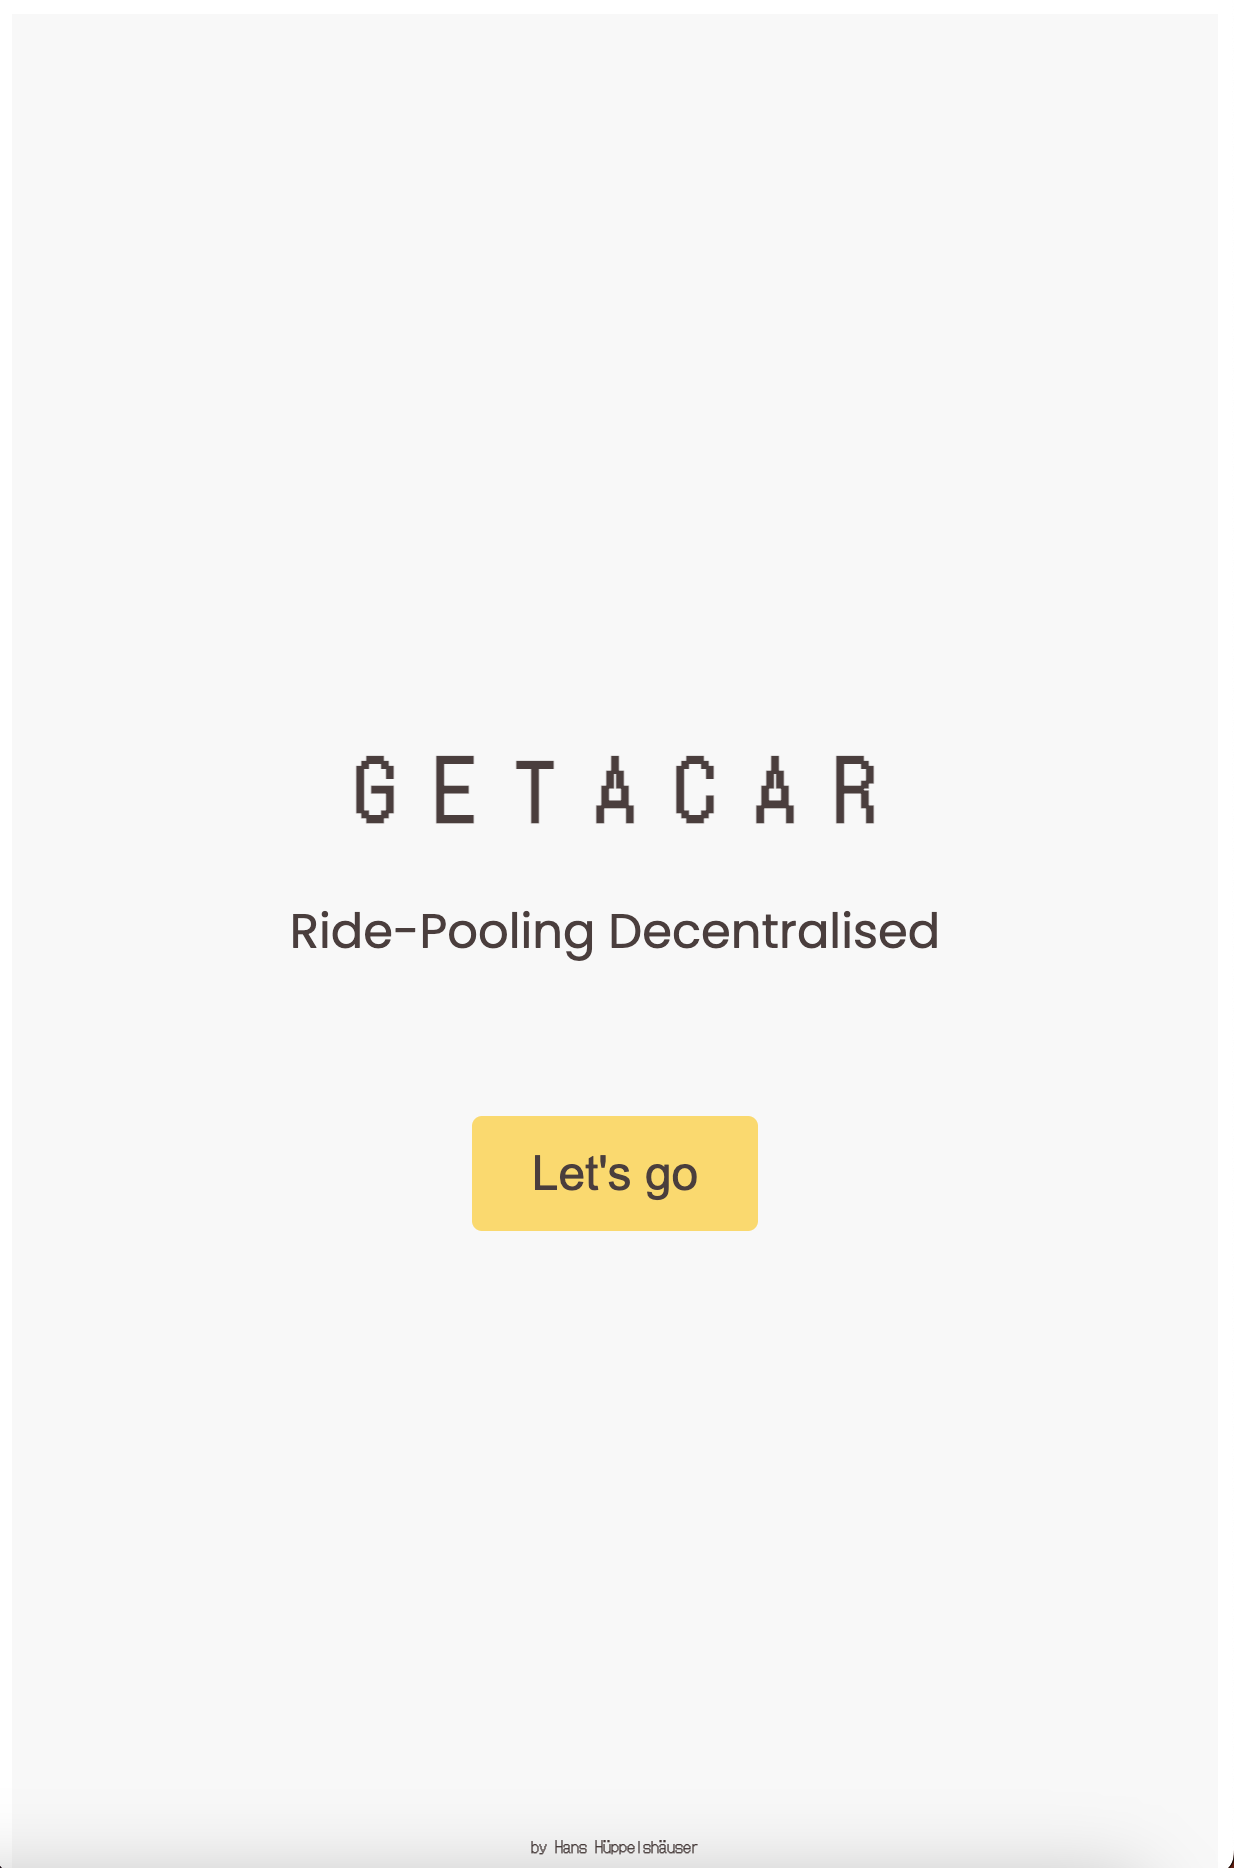
\includegraphics[width=\linewidth]{data/ffss/1.png}
        \caption{Frontend: Welcome Screen}
        \label{fig:WelcomeScreen}
    \end{minipage}
    \hfill
    \begin{minipage}{0.45\linewidth}
        \centering
        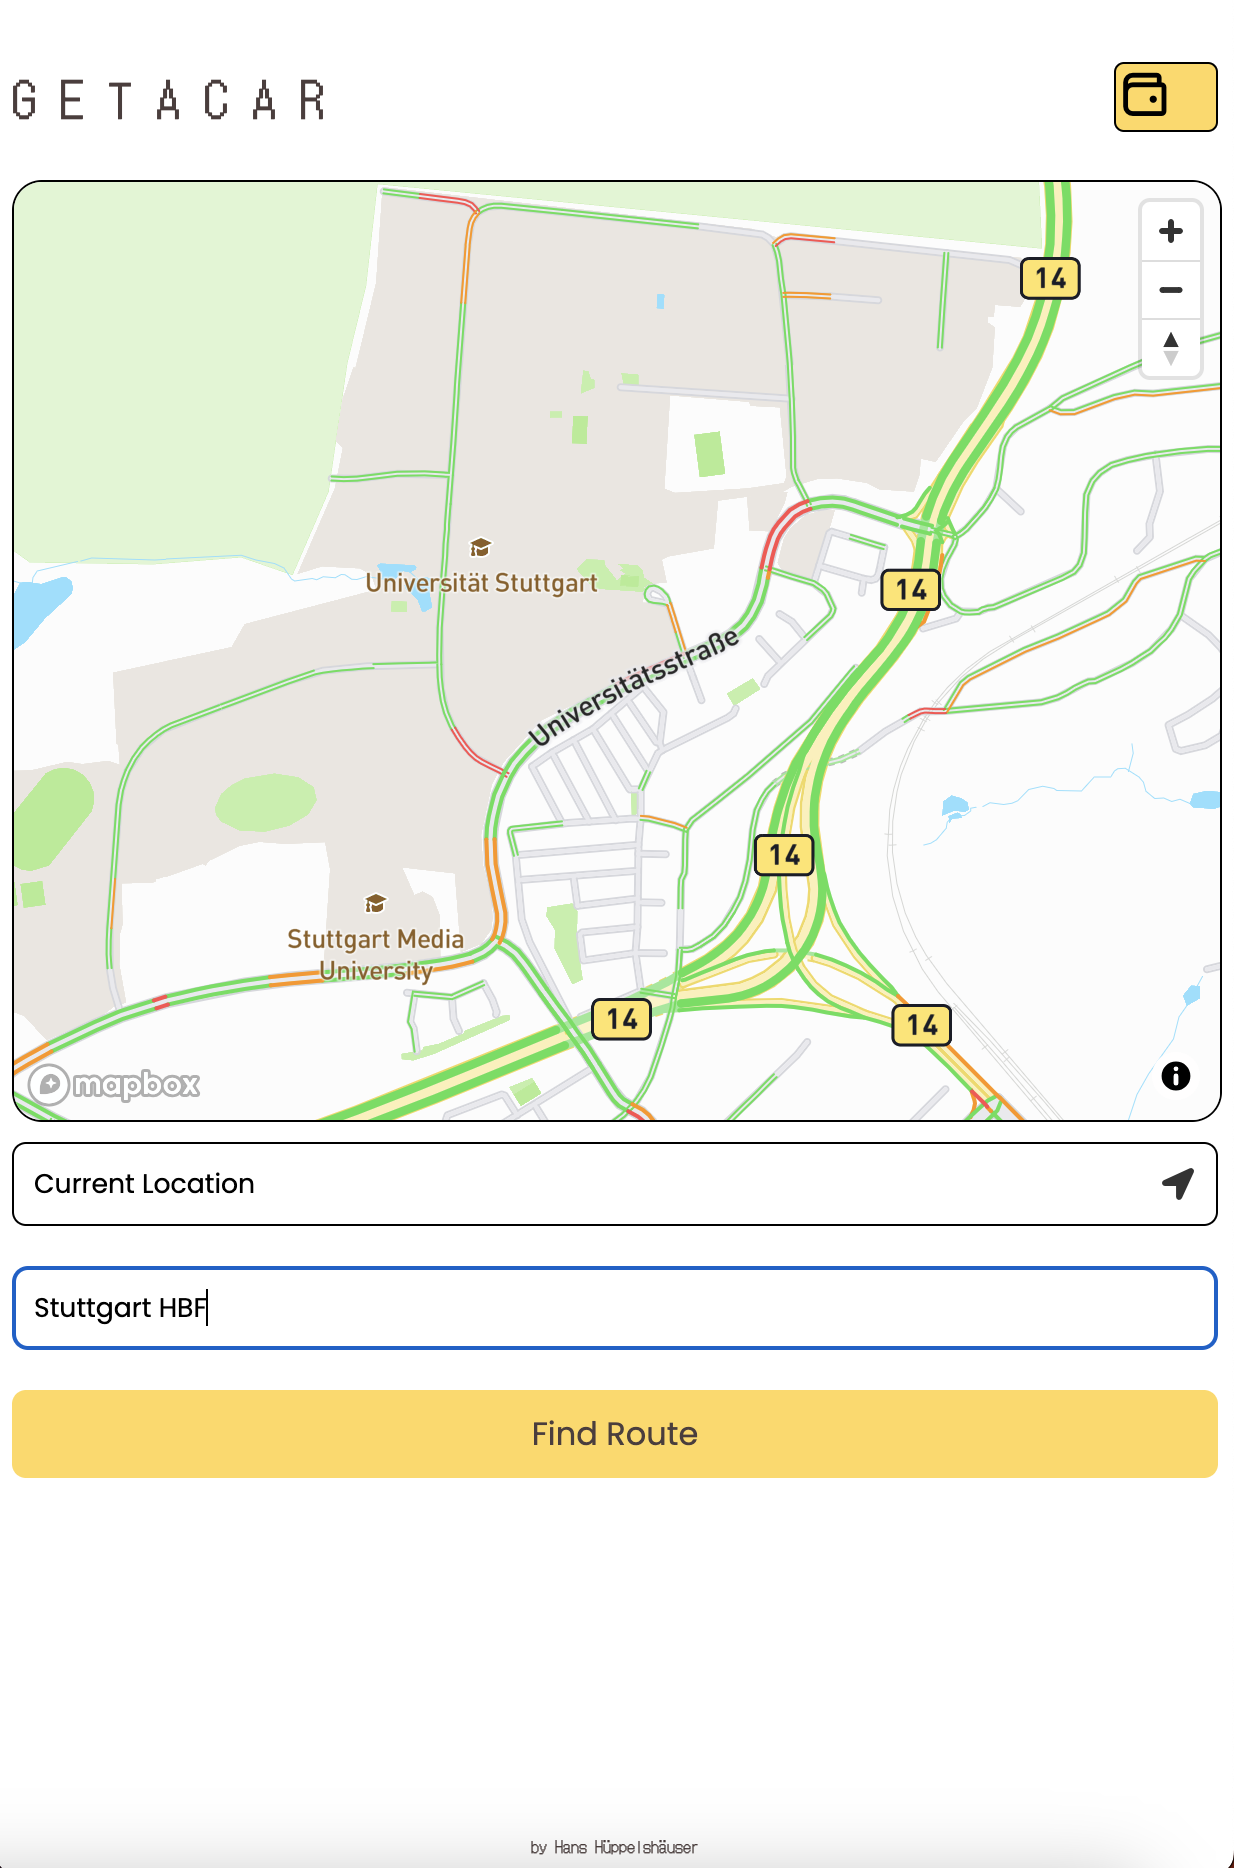
\includegraphics[width=\linewidth]{data/ffss/2.png}
        \caption{Frontend: Map Screen}
        \label{fig:MapScreen}
    \end{minipage}
    
\end{figure}

After the customer presses the ''Find Route'' button, they will be presented with a preview of their trip, including some additional information like the expected duration and distance of the travel. The customer now has the possibility to post a ride request by pressing the ''Request Ride'' button, as shown in \ref{fig:MapTripScreen}.
This will send a ride request to the matching service (that was suggested through the matching smart contract). As long as the auction is running on the matching service, the customer frontend will display the loading screen seen in \ref{fig:SearchRideScreen}.


\begin{figure}[H]
    \centering
    
    \begin{minipage}{0.45\linewidth}
        \centering
        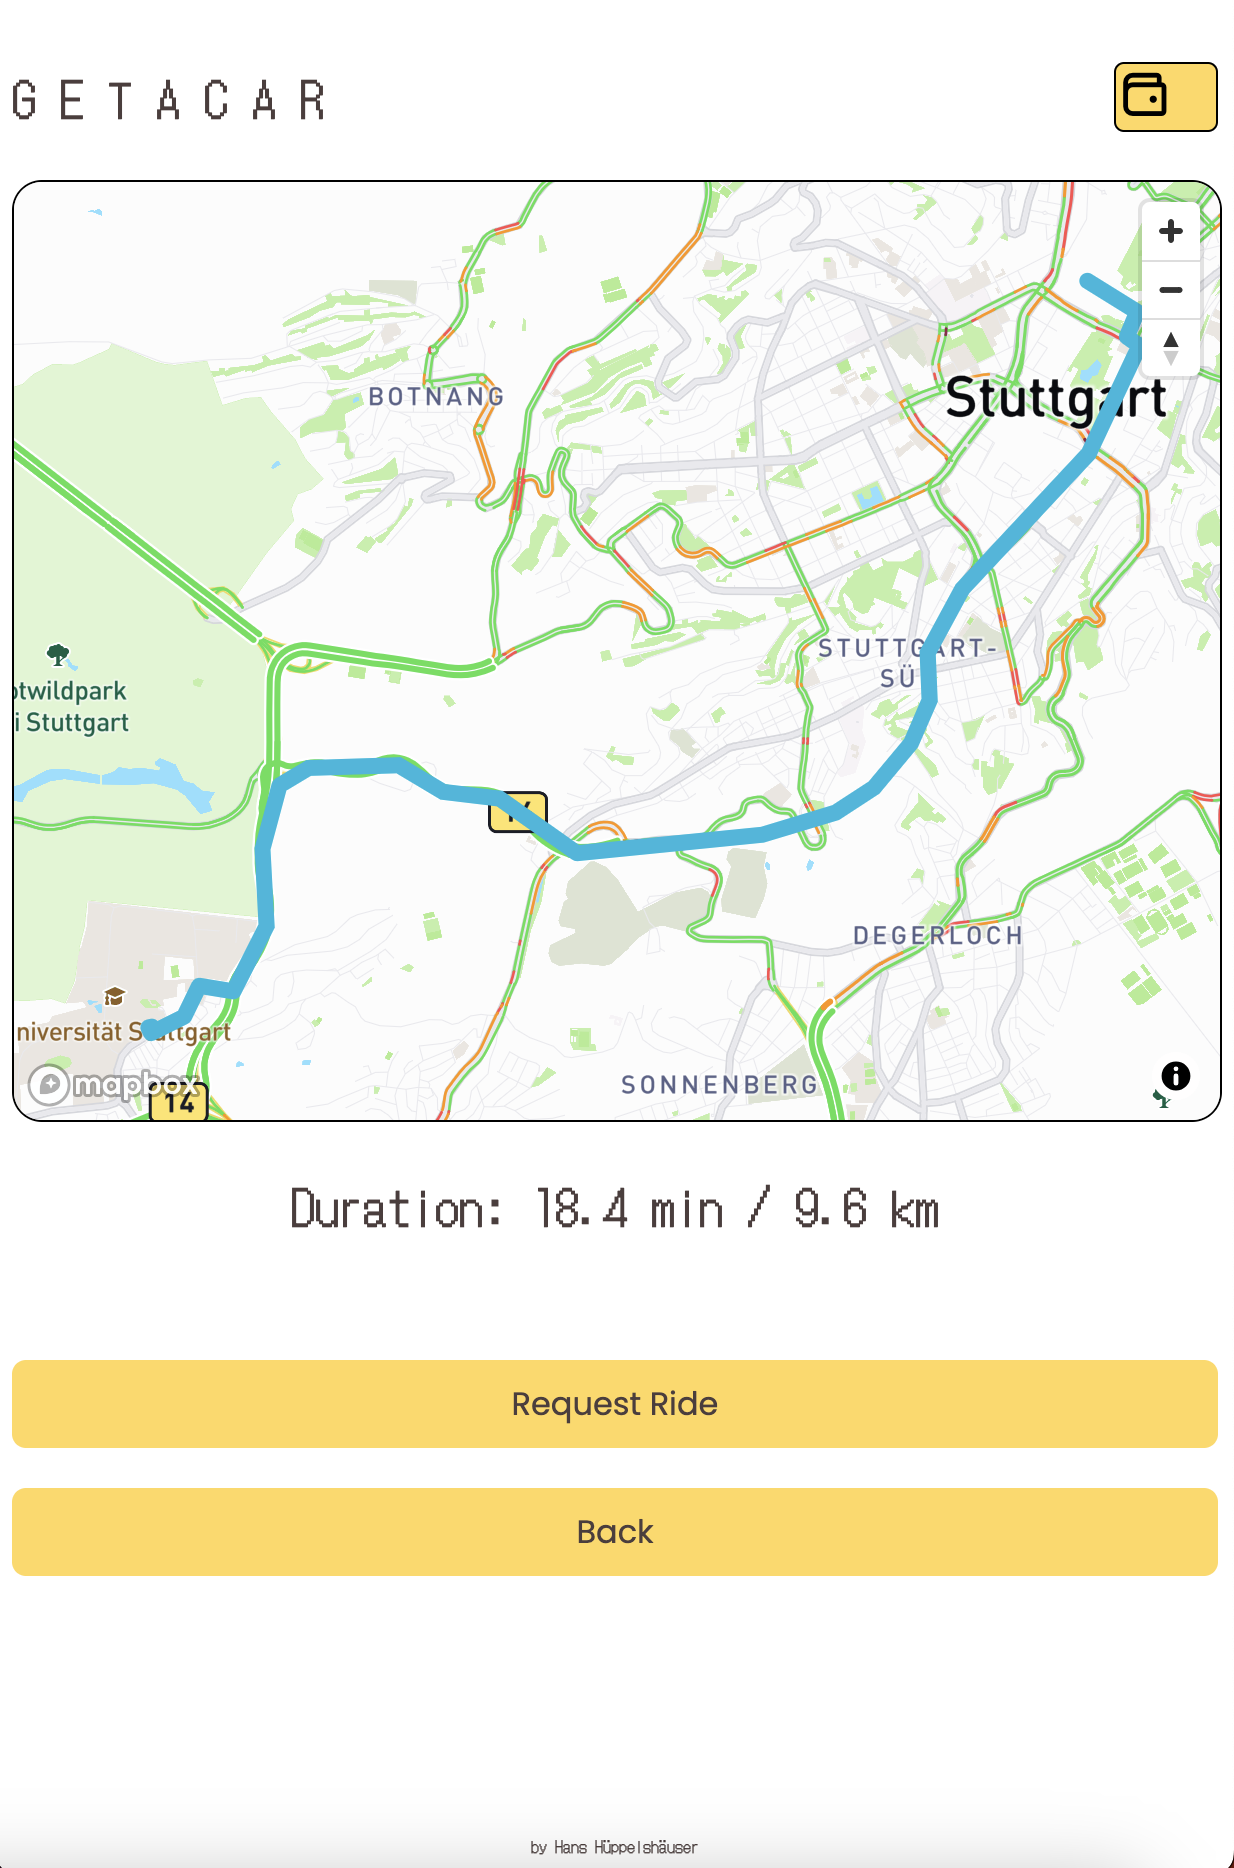
\includegraphics[width=\linewidth]{data/ffss/3.png}
        \caption{Frontend: Map Trip Screen}
        \label{fig:MapTripScreen}
    \end{minipage}
    \hfill
    \begin{minipage}{0.45\linewidth}
        \centering
        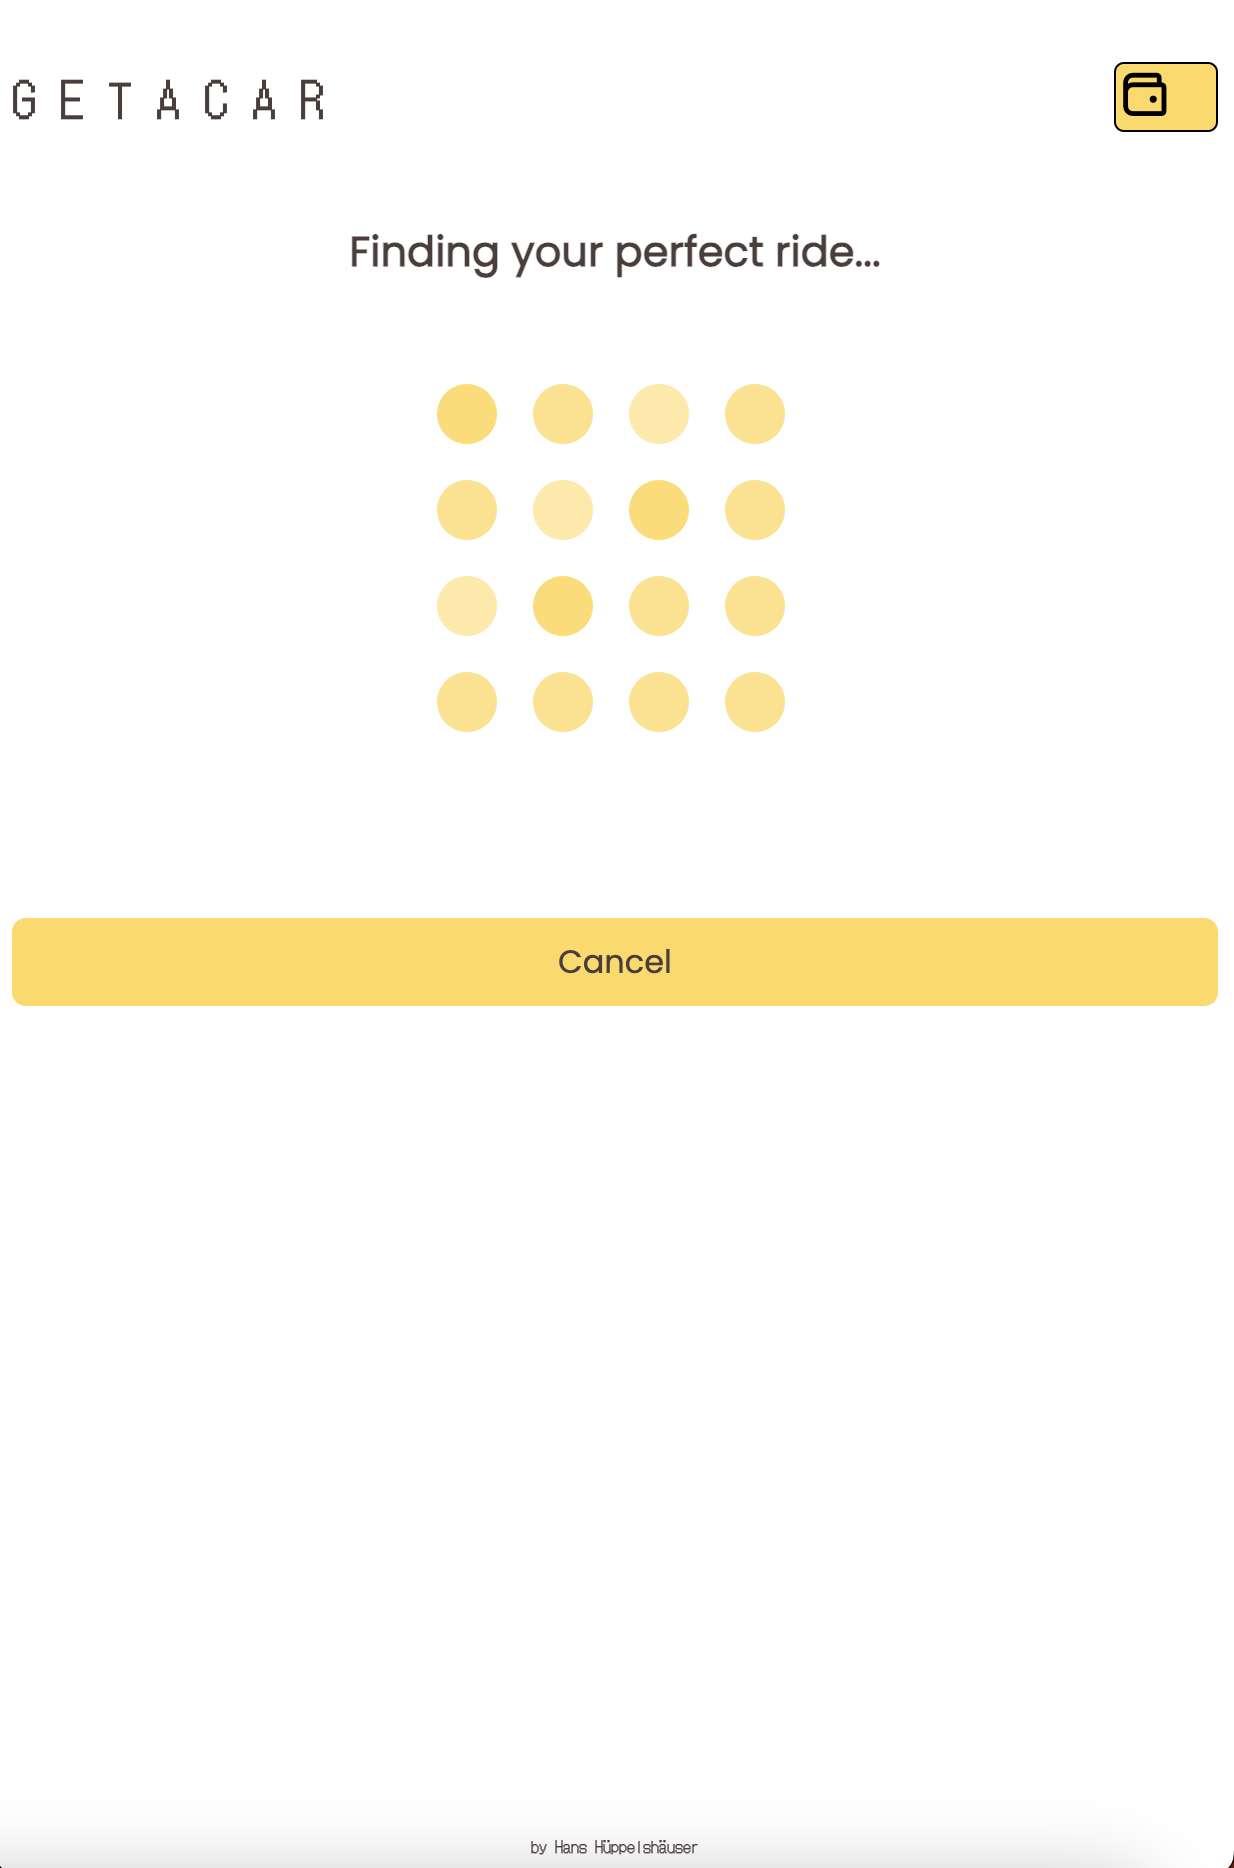
\includegraphics[width=\linewidth]{data/ffss/4.png}
        \caption{Frontend: Search Ride Screen}
        \label{fig:SearchRideScreen}
    \end{minipage}
    
\end{figure}

Once the auction is closed, the customer is presented the winning bid with all the important information about the ride, as shown in \ref{fig:RideOverviewScreen}. In the top right corner, a timer counts down the time that is left before the offer expires. As long as the offer has not expired, the customer is able to press the ''Book Ride'' button to confirm the ride and thereby create a ride contract on the blockchain. The frontend also has dedicated screens that inform the customer if the matching service could not find a ride or if the offer expired because the customer did not press the ''Book Ride'' button.

After a ride is found and the customer confirms the ride, the frontend changes into the on-ride view that provides status updates about all activities happening on the ride and tracks them via the ride contract. Screen \ref{fig:AwaitingConfirmationScreen} shows the ''waiting Confirmation Screen''. At this stage, the frontend monitors the blockchain and waits for the event from the ride contract that signals that the ride provider has co-signed the ride contract.


\begin{figure}[H]
    \centering
    
    \begin{minipage}{0.45\linewidth}
        \centering
        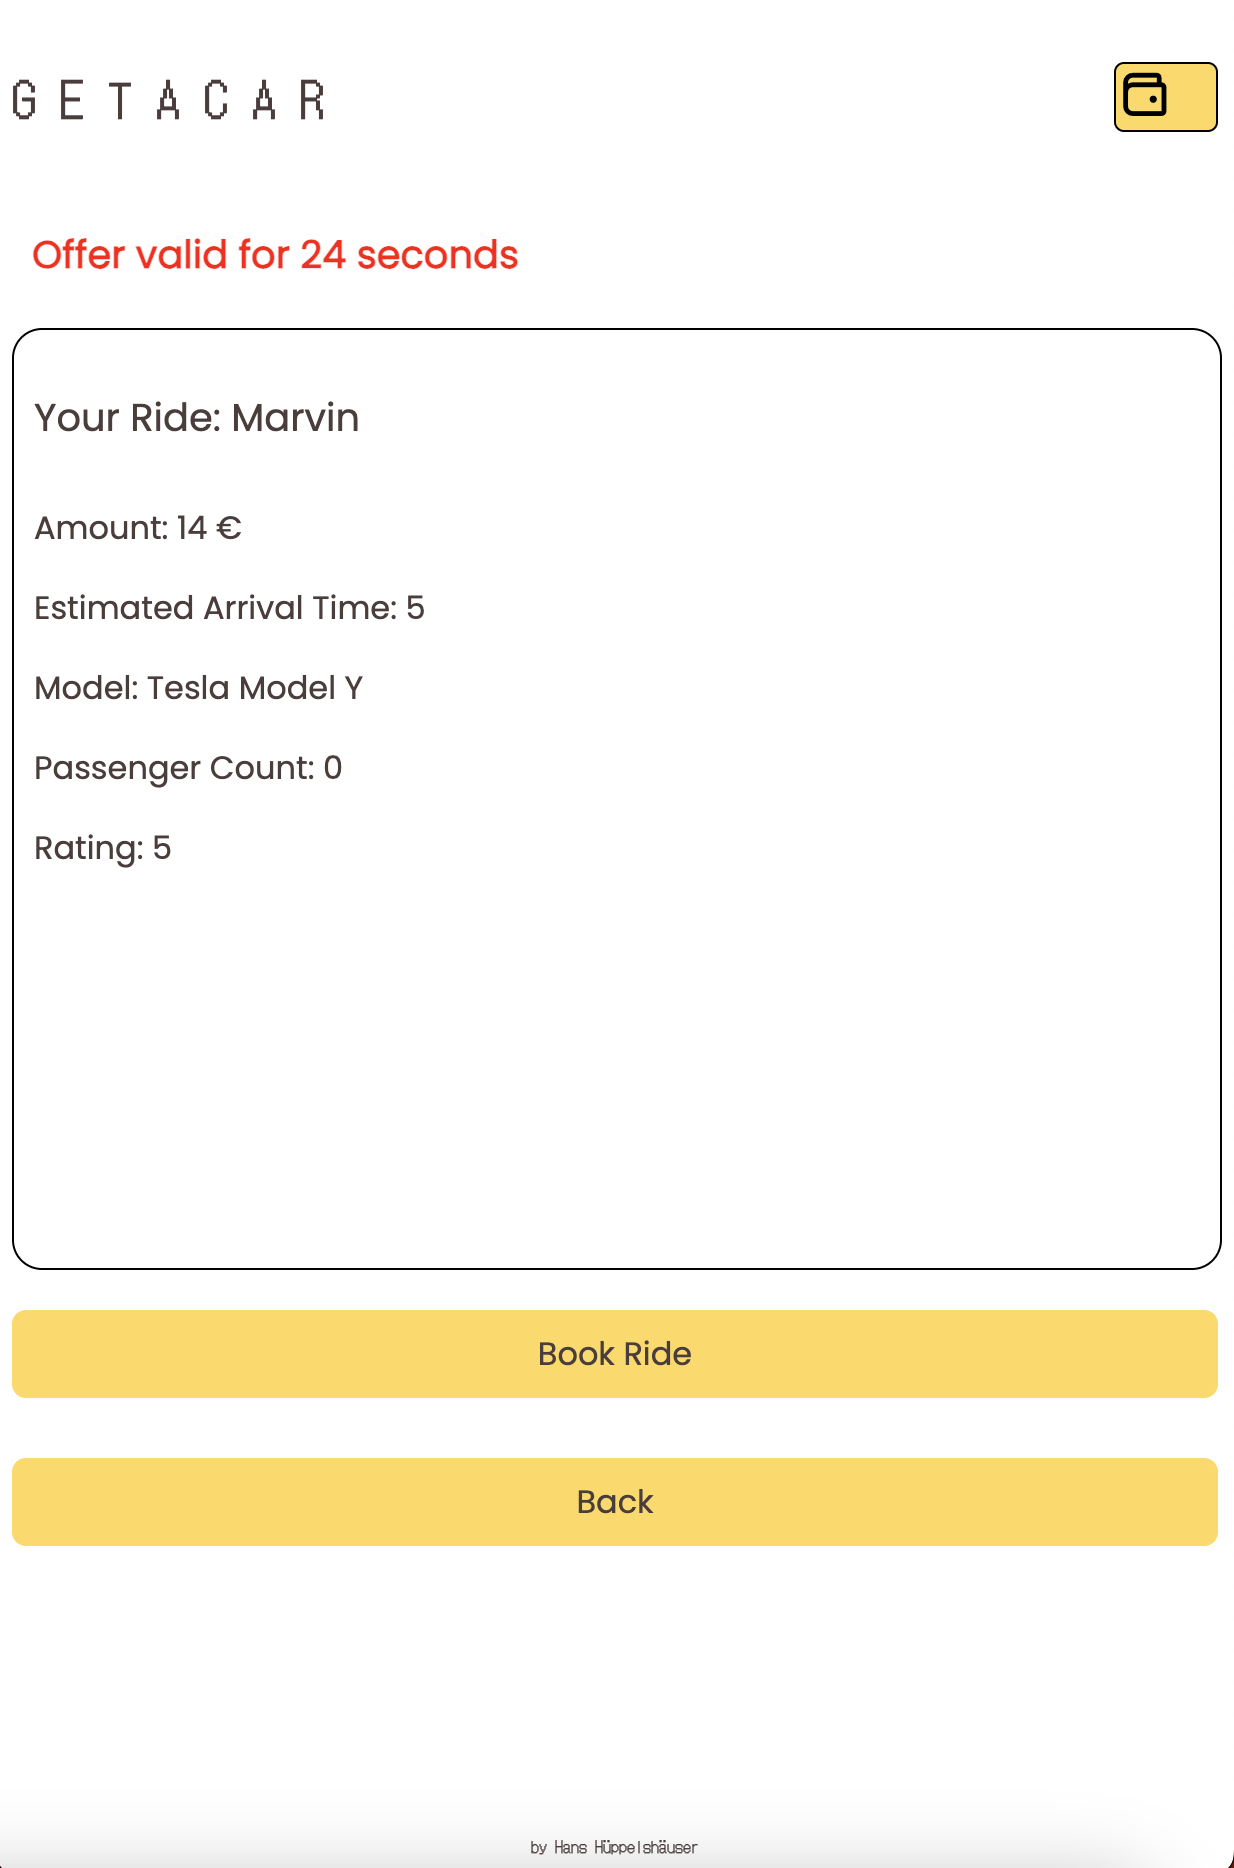
\includegraphics[width=\linewidth]{data/ffss/5.png}
        \caption{Frontend: Ride Overview Screen}
        \label{fig:RideOverviewScreen}
    \end{minipage}
    \hfill
    \begin{minipage}{0.45\linewidth}
        \centering
        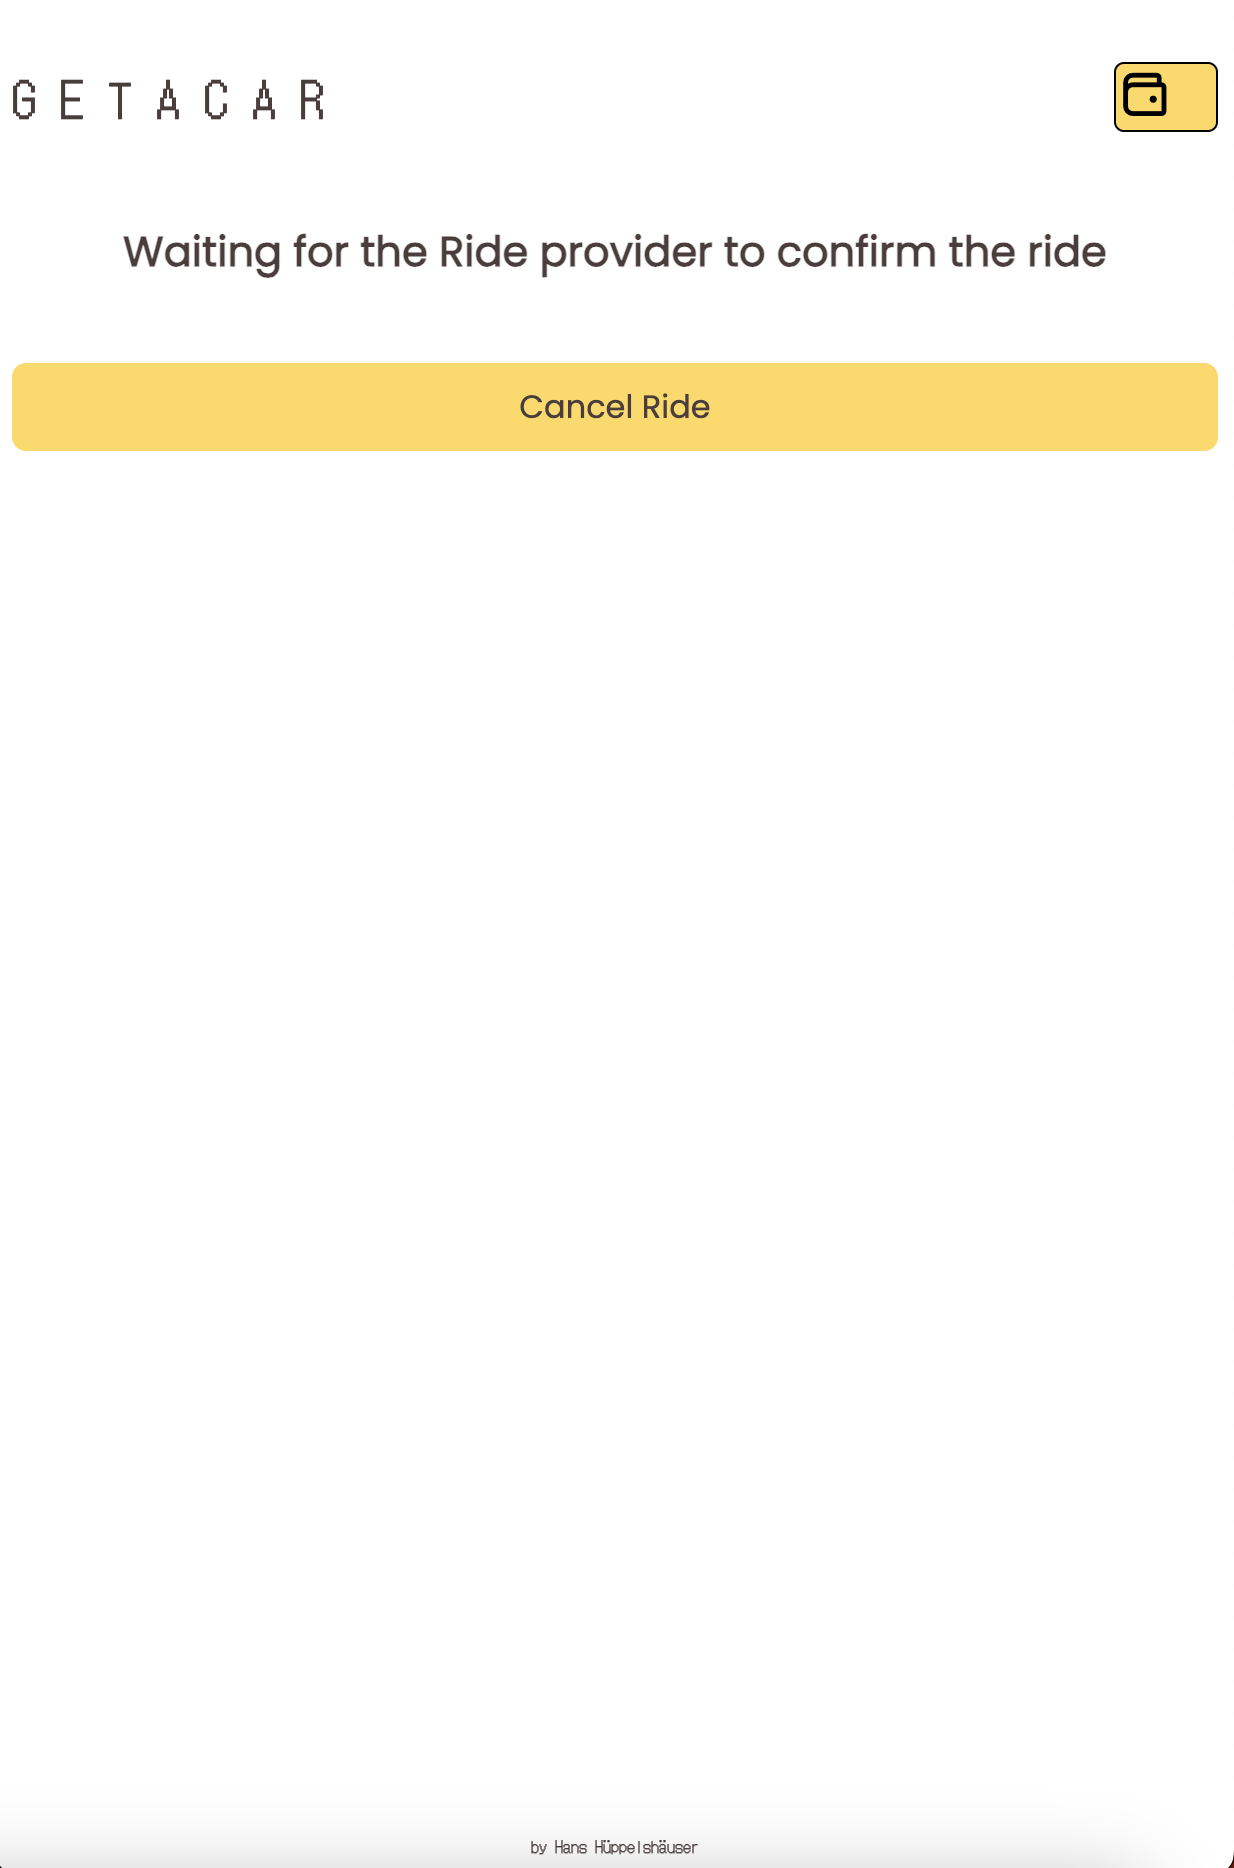
\includegraphics[width=\linewidth]{data/ffss/6.png}
        \caption{Frontend: Awaiting Confirmation Screen}
        \label{fig:AwaitingConfirmationScreen}
    \end{minipage}
    
\end{figure}

When the ride provider has signed the contract and confirmed that they started driving to the agreed pickup location, the on-ride screen changes to display the new status of the ride, as seen in \ref{fig:PickupLocationDriveScreen}. A market-ready version of the platform would also show the live position of the ride provider to the customer that the ride provider has shared as an encrypted message through the ride contract. However, this feature is not part of the prototype implementation as the prototype only utilises virtual vehicles as ride providers that are not able to provide real-time GPS position updates.

Once the ride provider has arrived at the pickup location and posted this update on the ride contract, the customer's frontend changes again to display the update, shown in \ref{fig:VehicleArrivedScreen}. The customer now enters the vehicle, and once they are ready to start their ride, they confirm this through the ''Start Driving'' button.


\begin{figure}[H]
    \centering
    
    \begin{minipage}{0.45\linewidth}
        \centering
        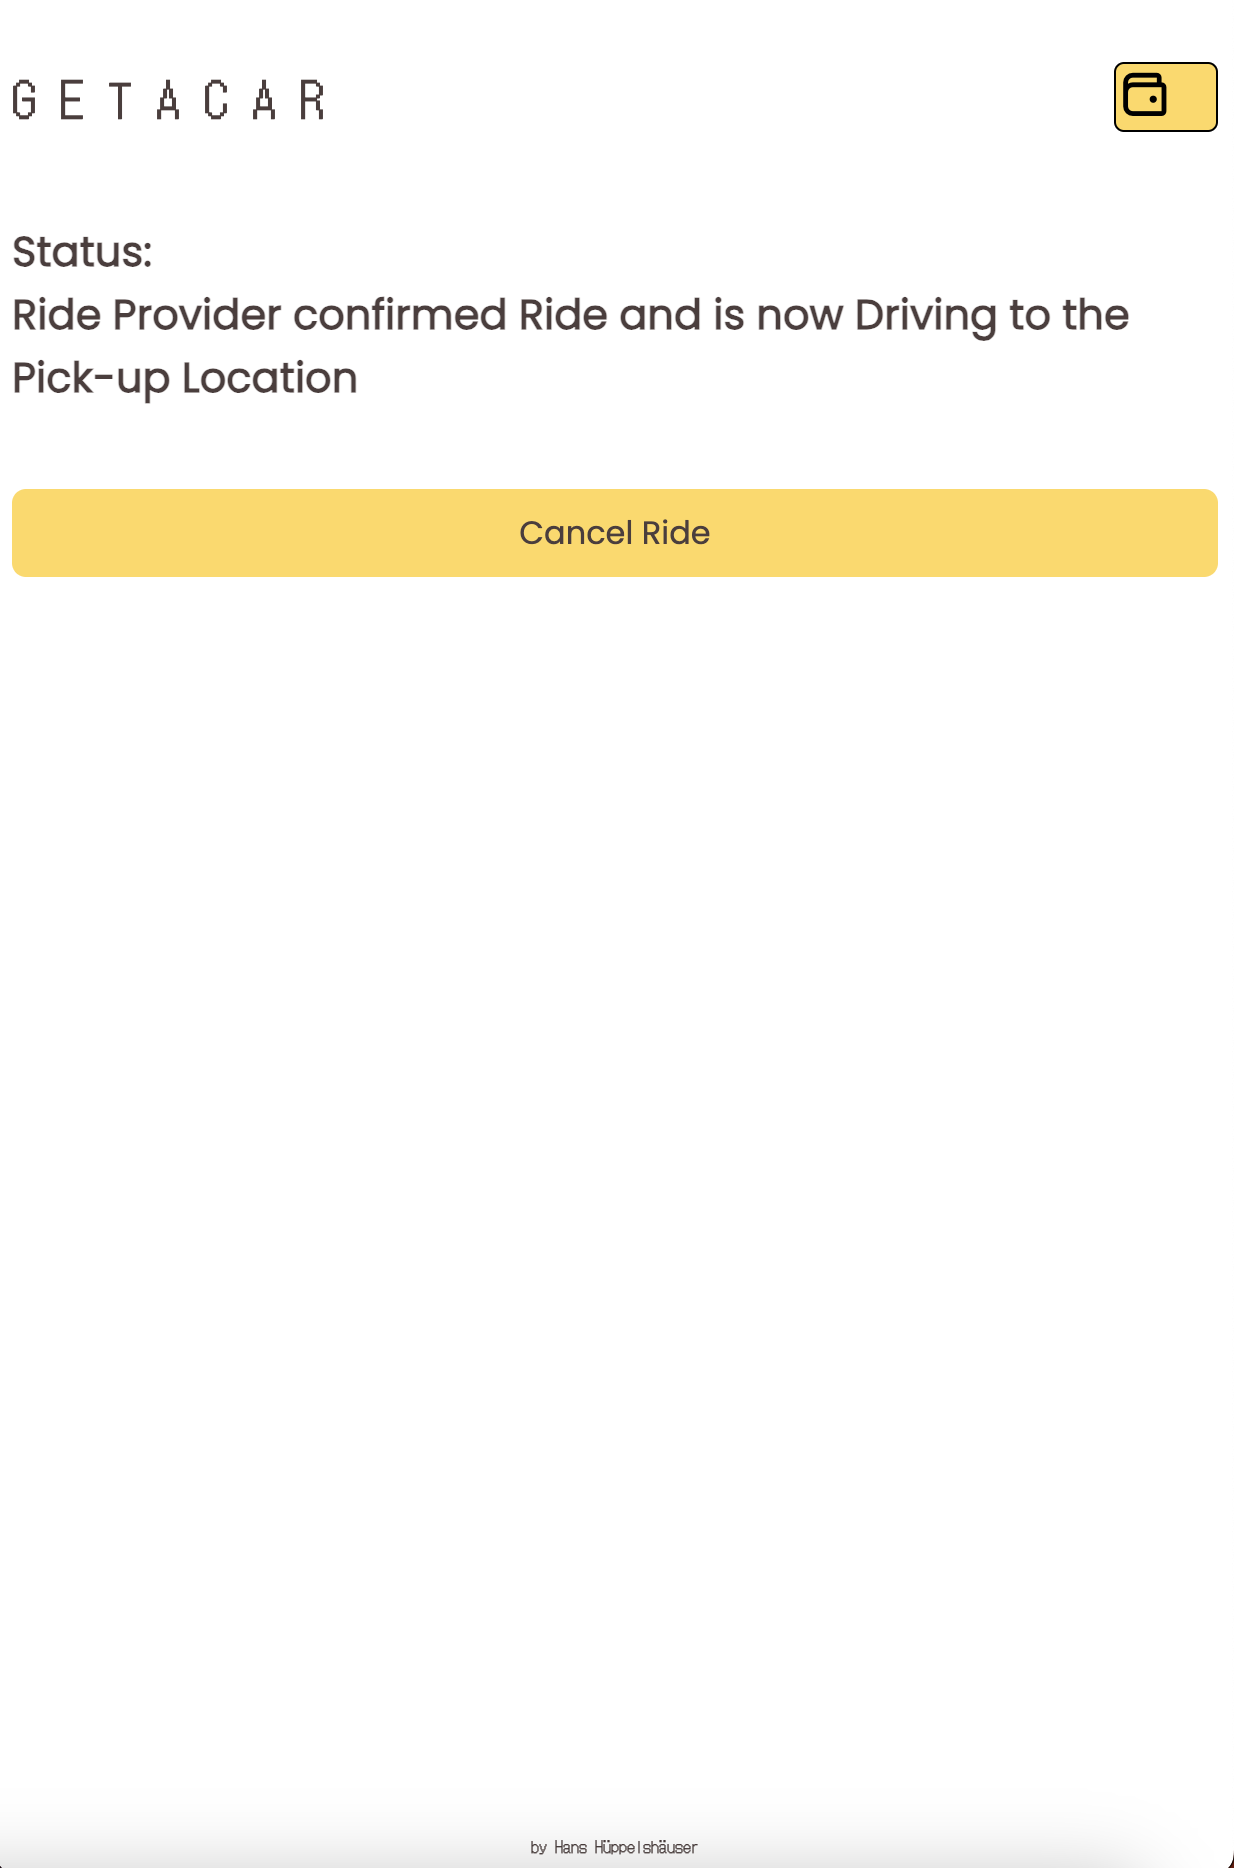
\includegraphics[width=\linewidth]{data/ffss/7.png}
        \caption{Frontend: Pickup Location Drive Screen}
        \label{fig:PickupLocationDriveScreen}
    \end{minipage}
    \hfill
    \begin{minipage}{0.45\linewidth}
        \centering
        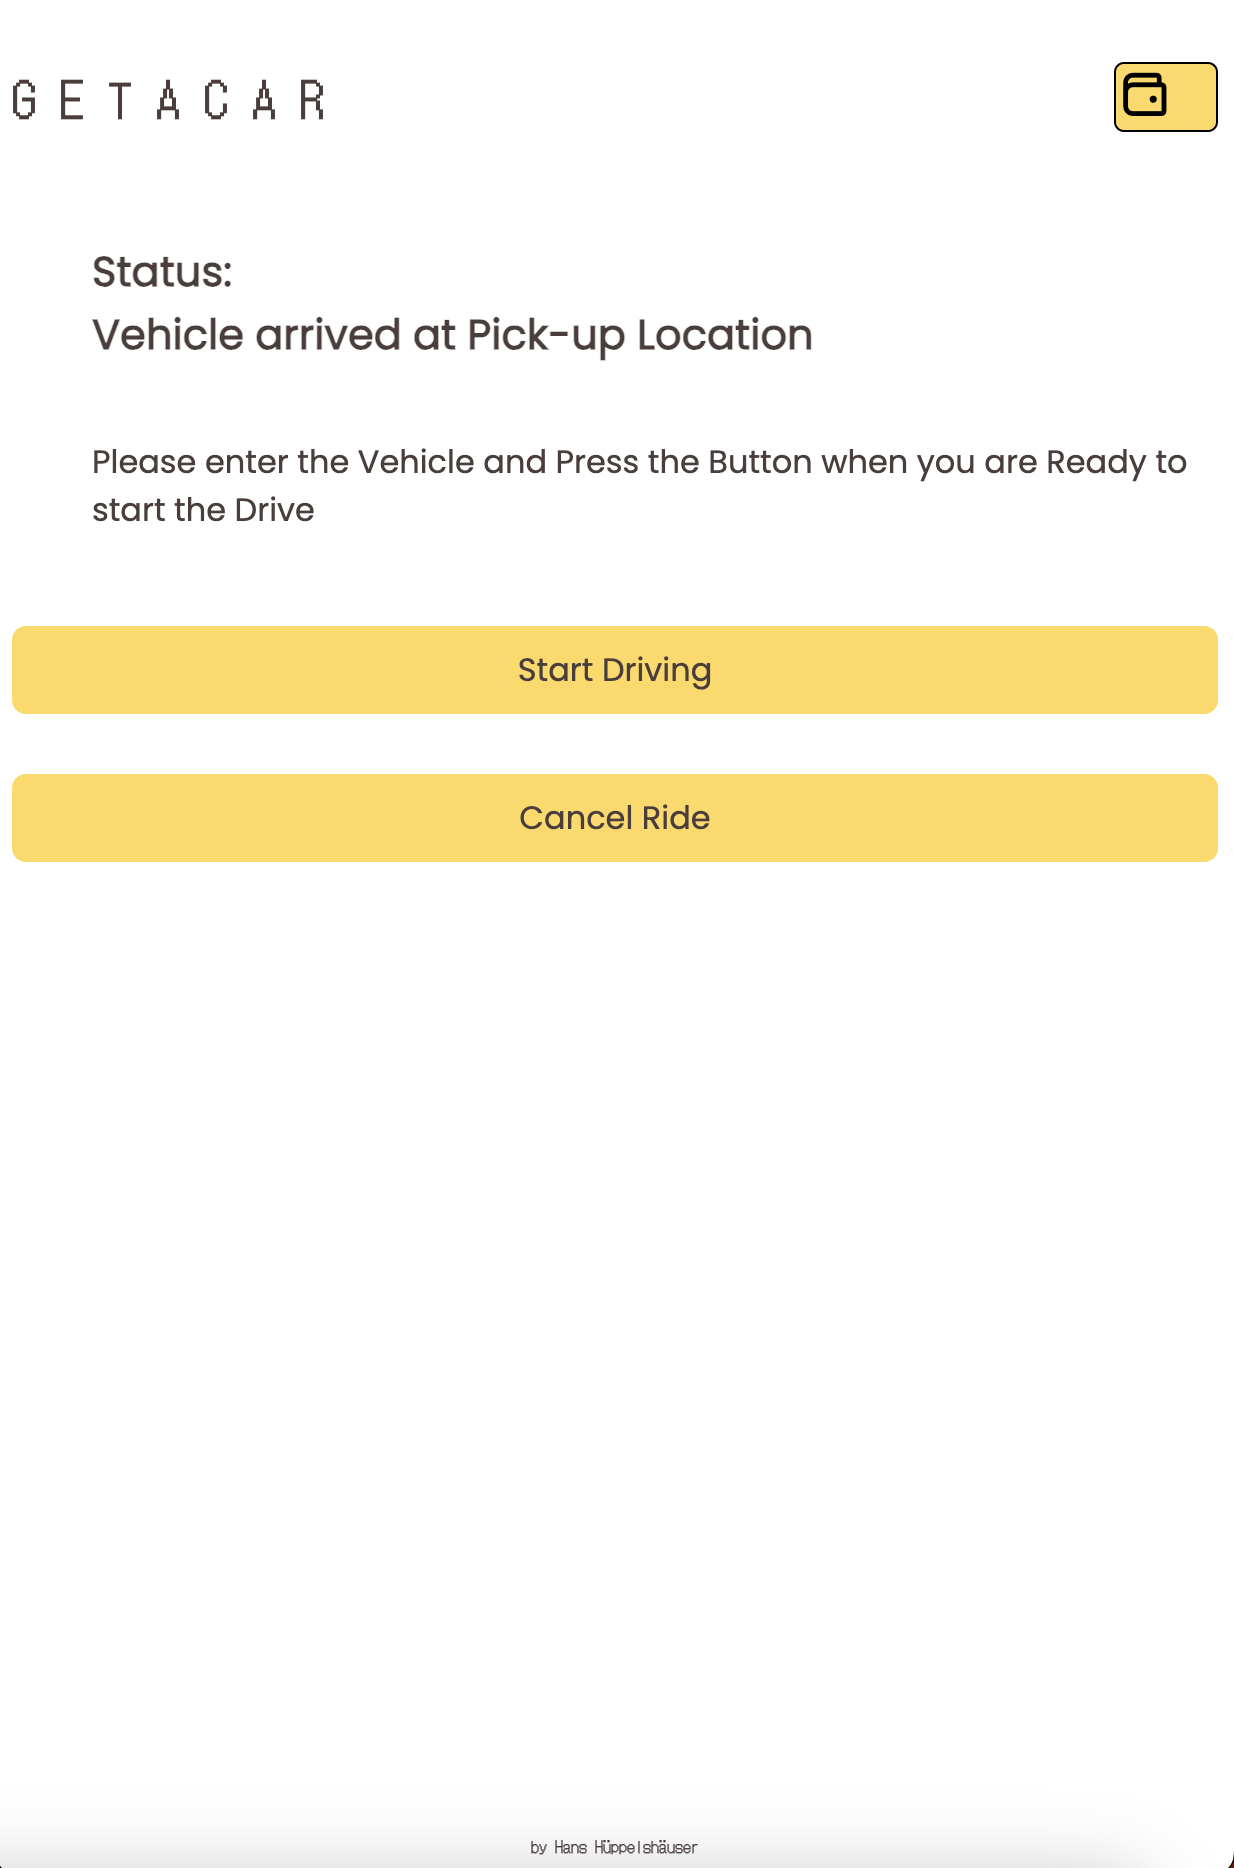
\includegraphics[width=\linewidth]{data/ffss/8.png}
        \caption{Frontend: Vehicle Arrived Screen}
        \label{fig:VehicleArrivedScreen}
    \end{minipage}
    
\end{figure}

After the ride provider has received the update from the customer that they are ready, the ride provider starts the ride to the destination. This is also represented via a status screen in the customer frontend, as shown in \ref{fig:DrivingScreen}. When arriving at the dropoff location, the ride provider posts this information onto the ride contract. The customer frontend notices this new event on the blockchain and updates the status of the frontend, as seen in \ref{fig:DestinationScreen}. On this screen, the customer has the possibility to confirm the ride completion and thereby end the ride process.

It is important to note that each status screen also provides a ''Cancel Ride'' button at all times that allows the customer to exit the ride process.

\begin{figure}[H]
    \centering
    
    \begin{minipage}{0.45\linewidth}
        \centering
        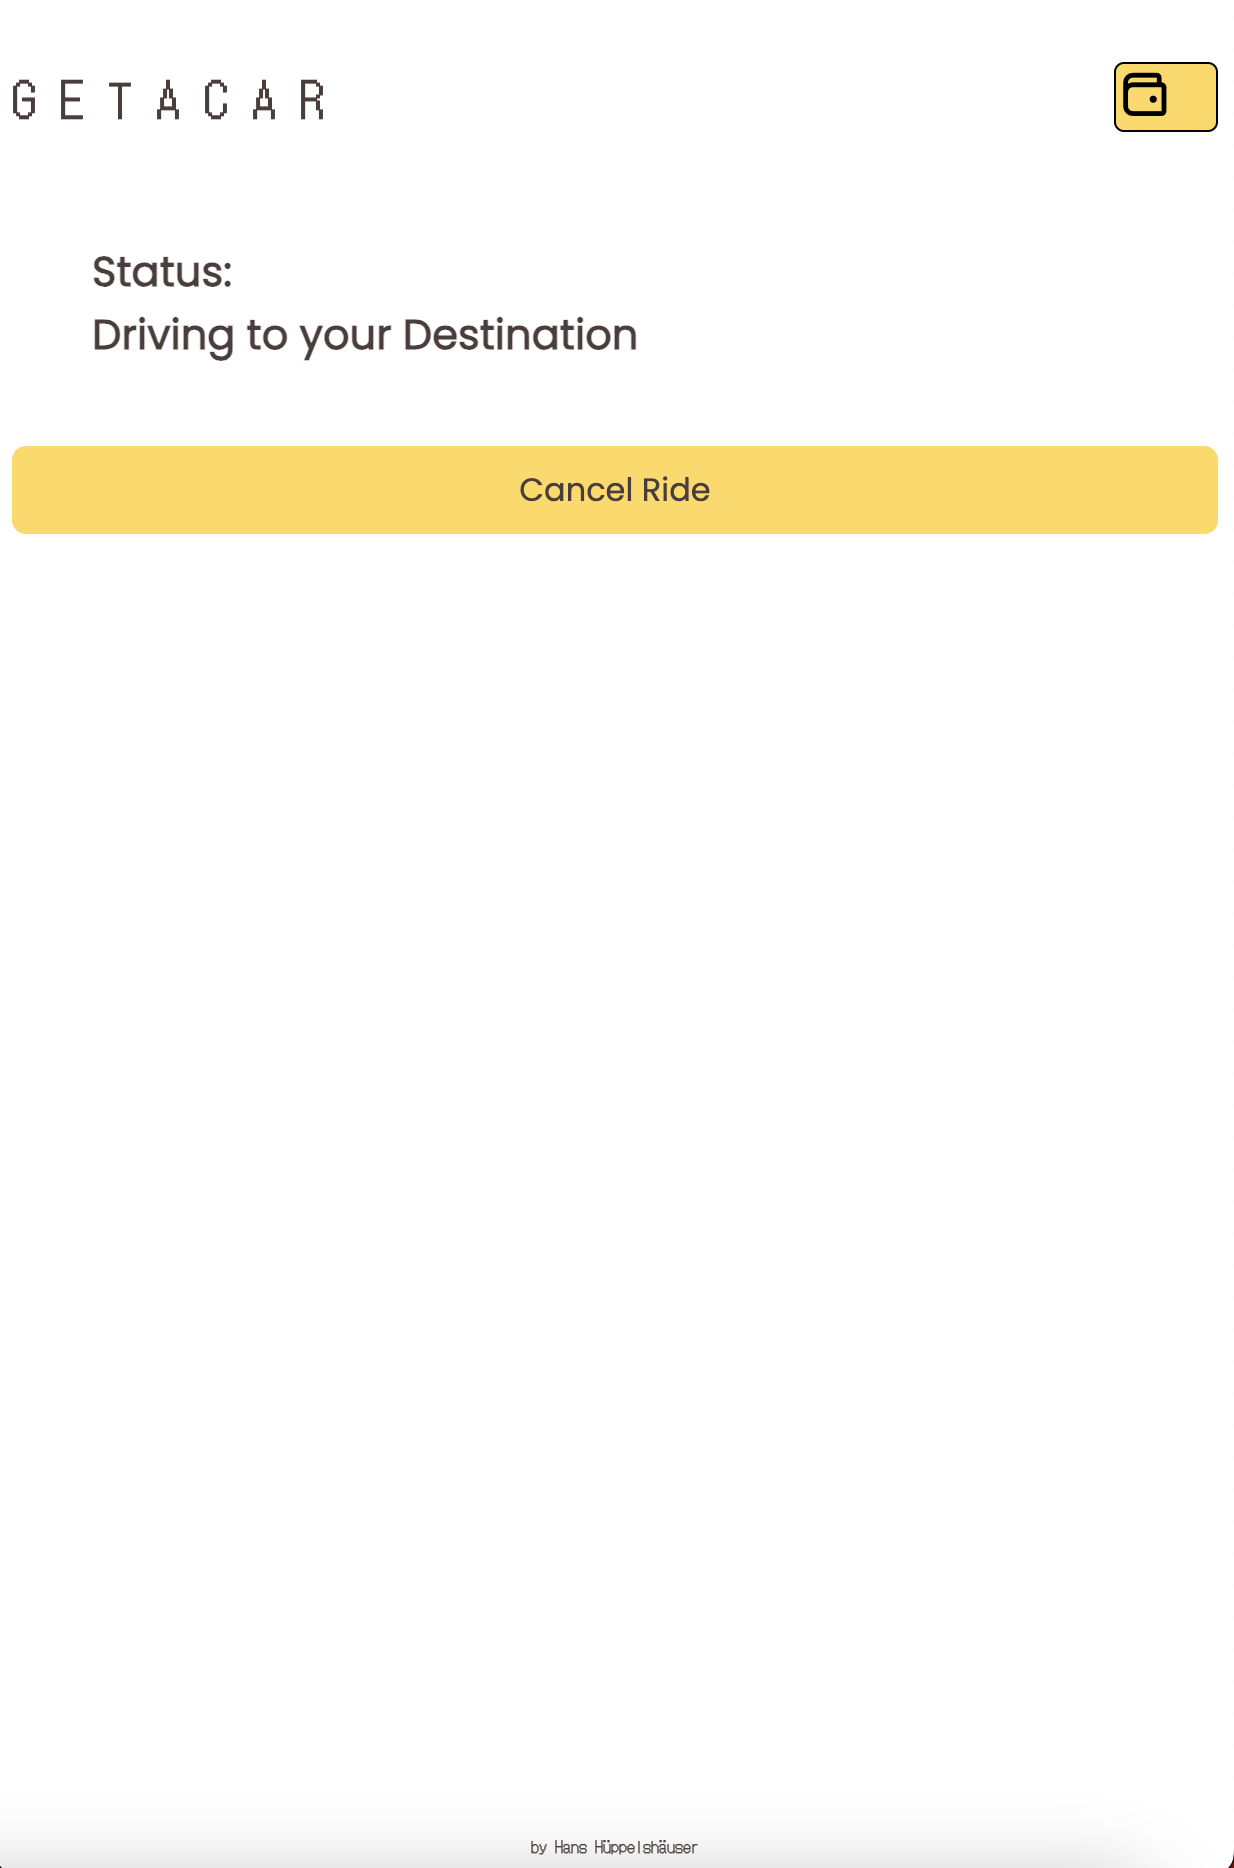
\includegraphics[width=\linewidth]{data/ffss/9.png}
        \caption{Frontend: Driving Screen}
        \label{fig:DrivingScreen}
    \end{minipage}
    \hfill
    \begin{minipage}{0.45\linewidth}
        \centering
        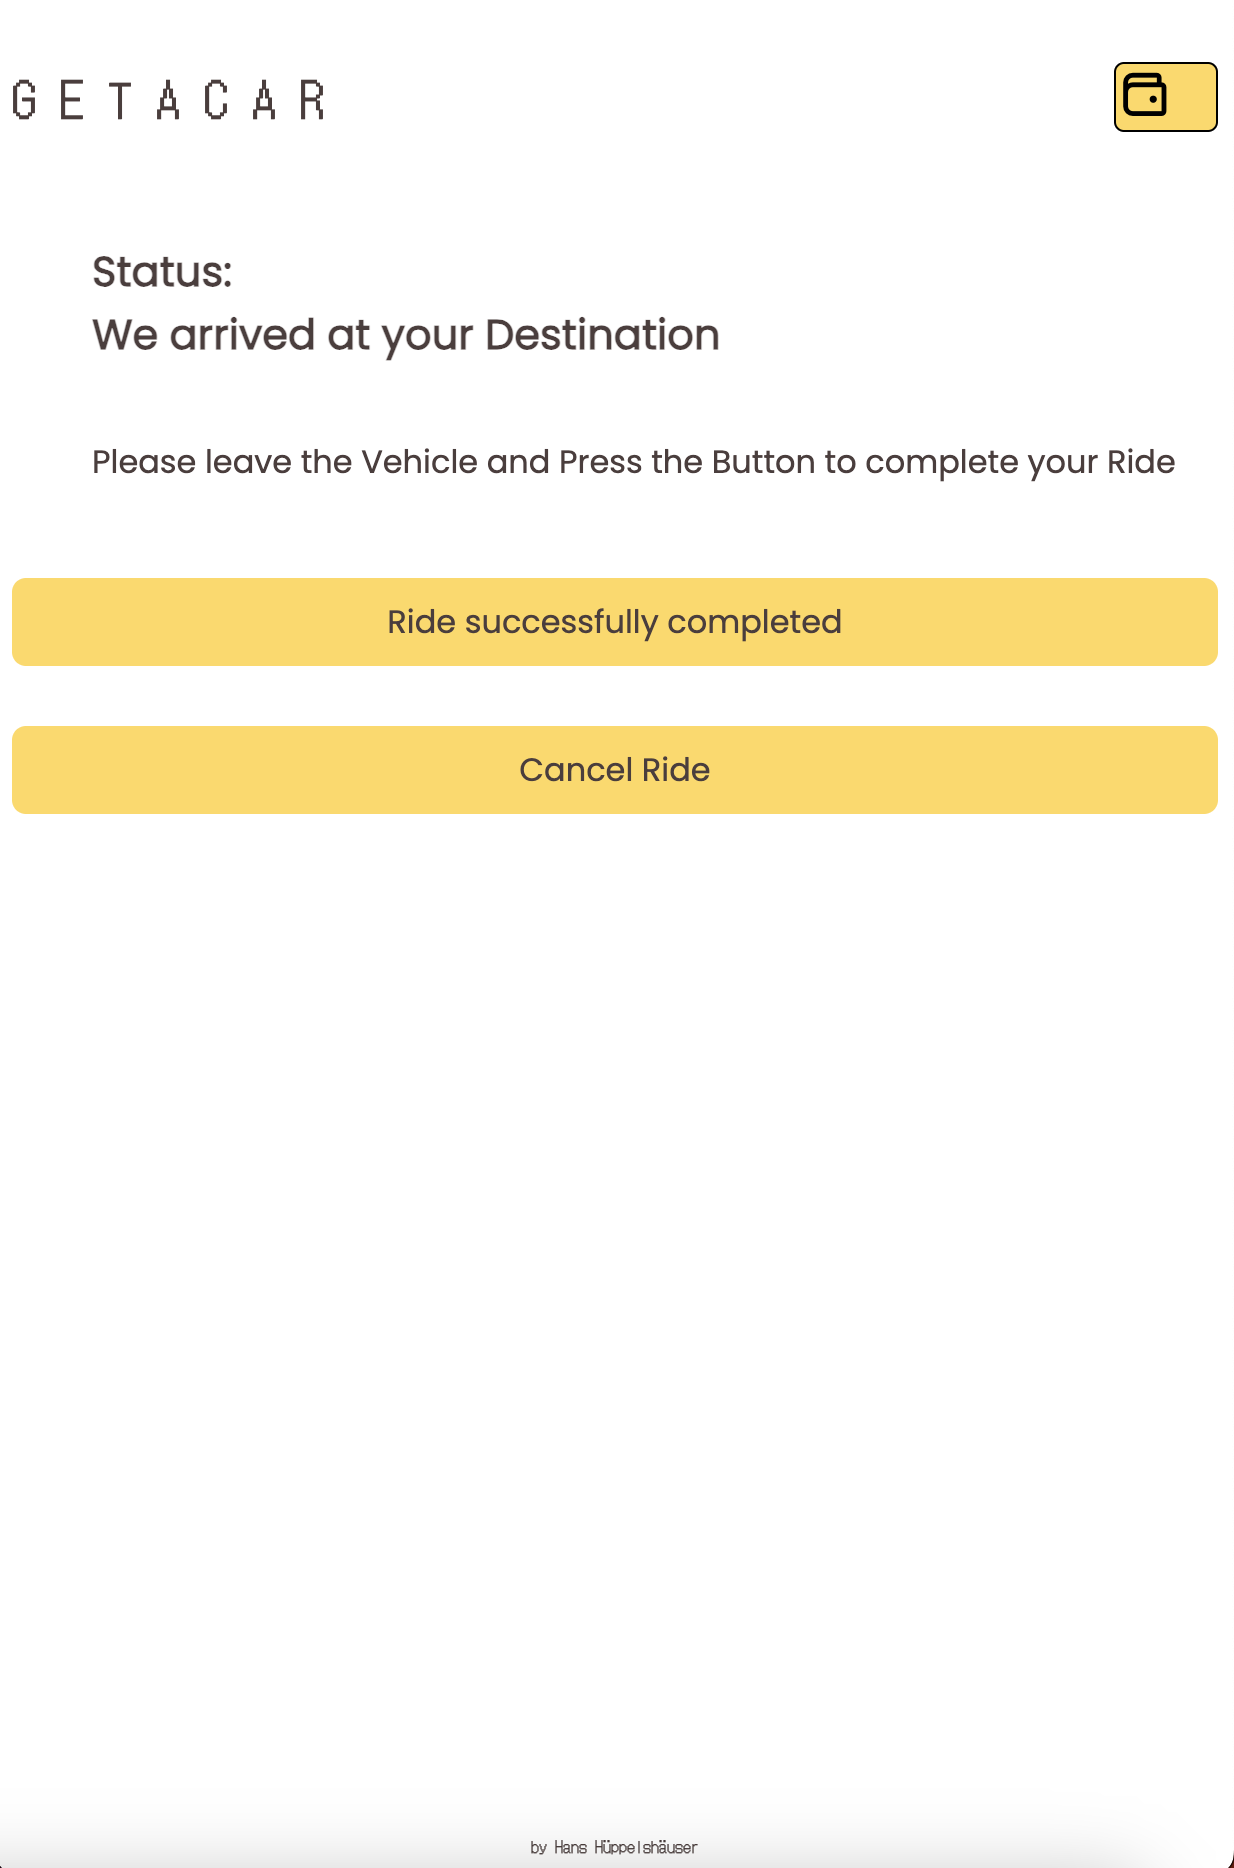
\includegraphics[width=\linewidth]{data/ffss/10.png}
        \caption{Frontend: Destination Screen}
        \label{fig:DestinationScreen}
    \end{minipage}
    
\end{figure}

Once the ride has ended, the customer is provided with a ''Ride Completed'' screen that allows the customer to rate the ride provider itself and their passengers, seen in \ref{fig:RateRideProviderScreen}. As described in \ref{subsec:RatingTrustMechanisms}, the problem with rating passengers is that no personal information should be exchanged through the platform about the passengers. This makes it complicated to ensure that the customer knows who is who when rating multiple passengers. To solve this problem, the ride provider shares the seating position and the start time of each passenger with the customer. The seating position is then visualised by the frontend, as seen in \ref{fig:RatePassengerScreen}. In this example, the passenger that is getting rated was sitting on seat number one, which is the seat on the front row on the left. 



\begin{figure}[H]
    \centering
    
    \begin{minipage}{0.45\linewidth}
        \centering
        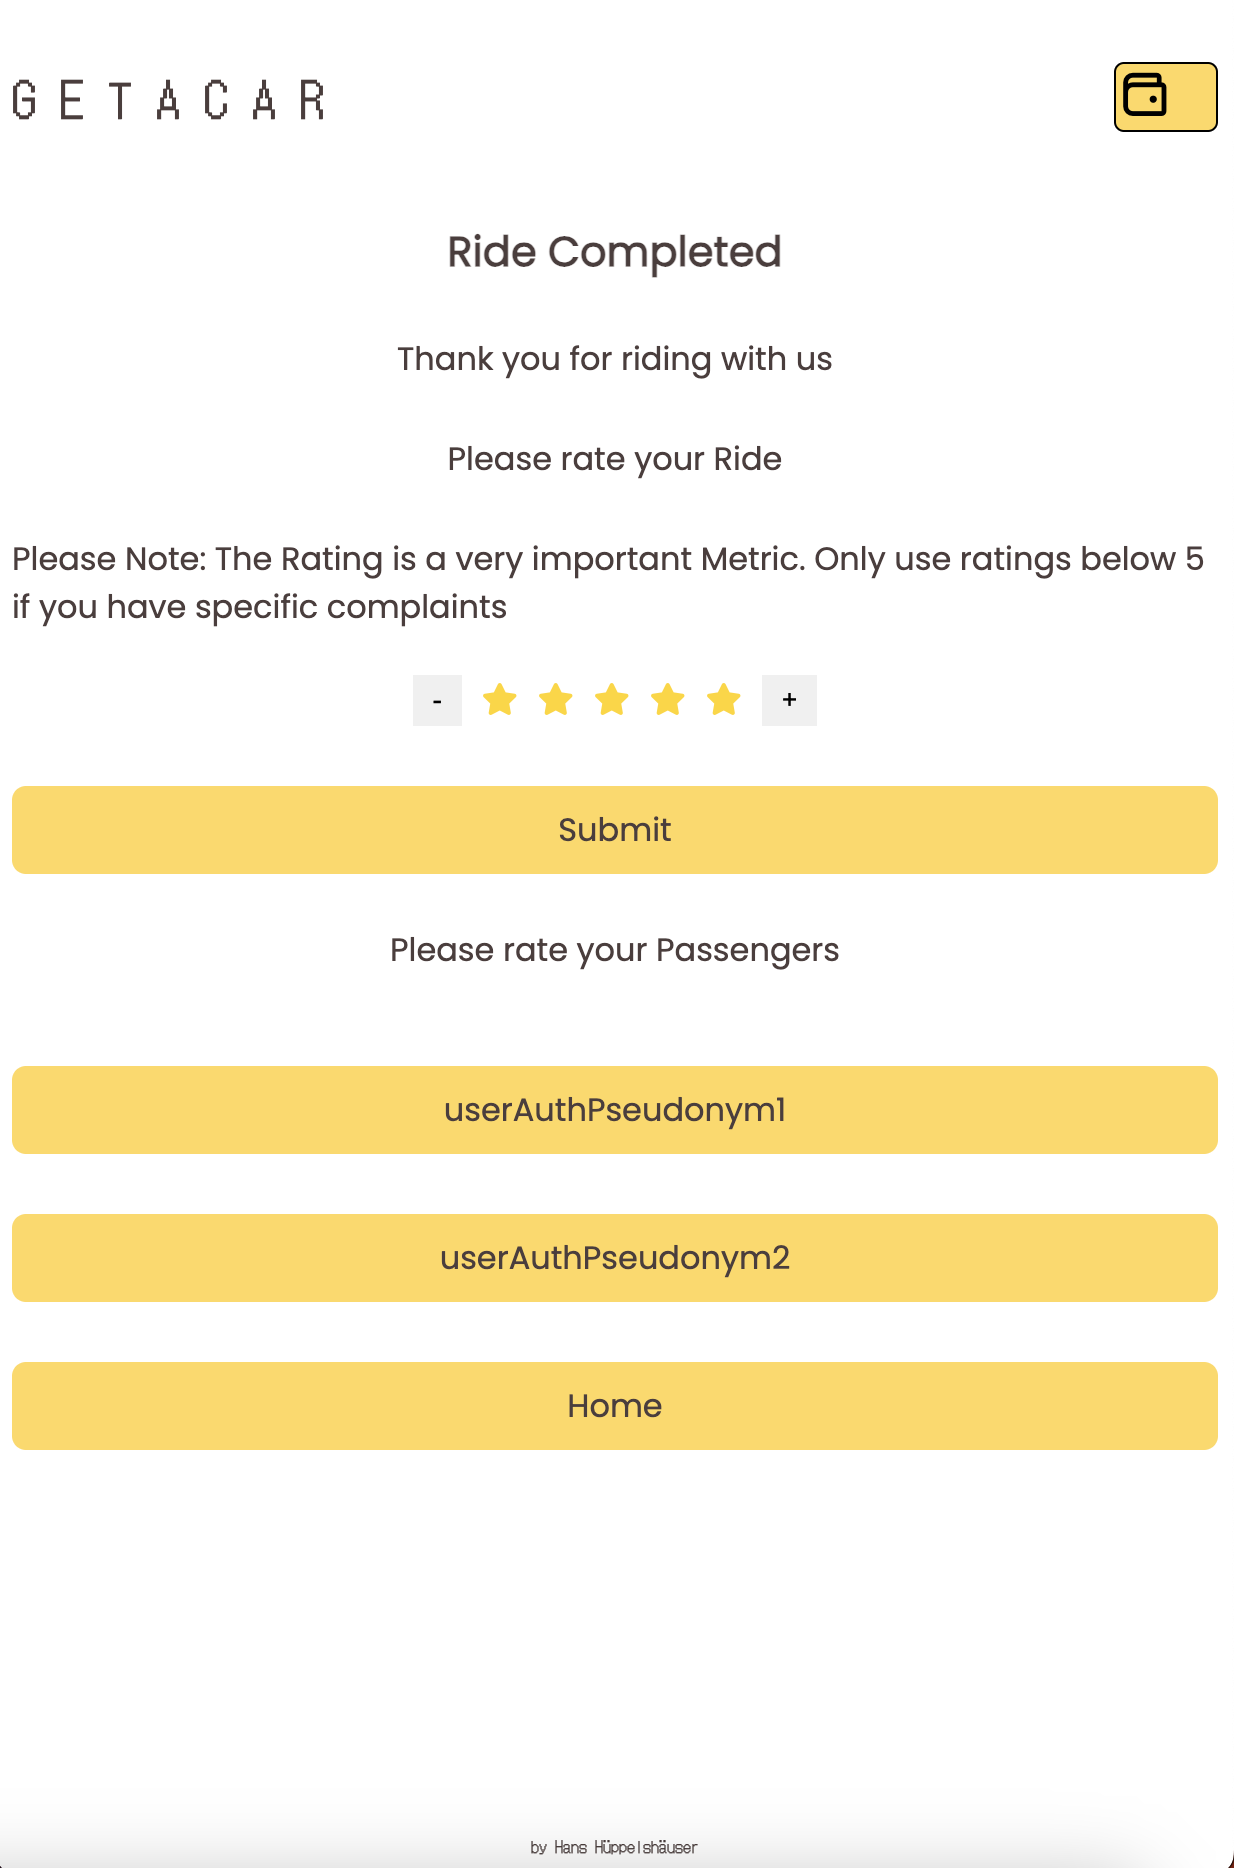
\includegraphics[width=\linewidth]{data/ffss/11.png}
        \caption{Frontend: Rate Ride Provider Screen}
        \label{fig:RateRideProviderScreen}
    \end{minipage}
    \hfill
    \begin{minipage}{0.45\linewidth}
        \centering
        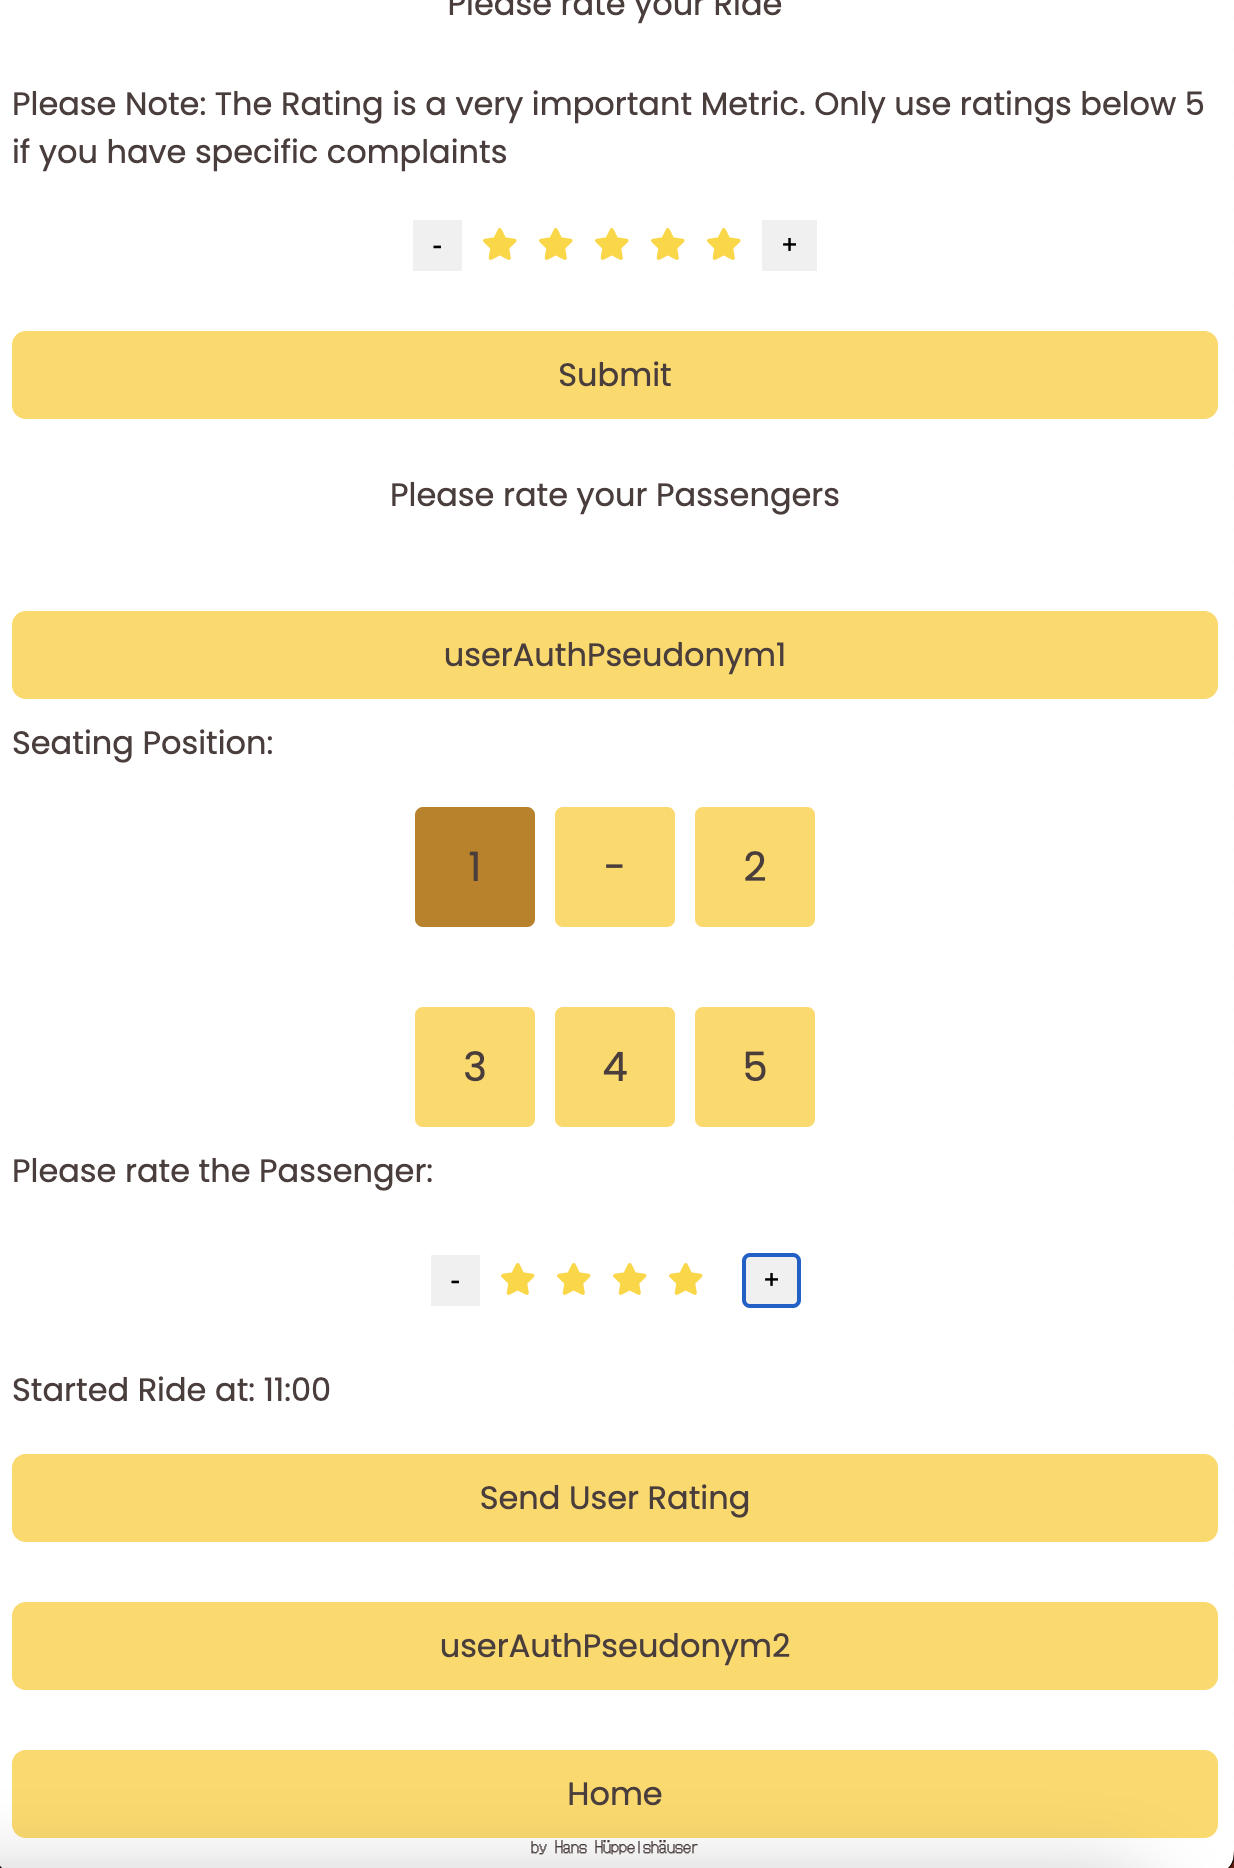
\includegraphics[width=\linewidth]{data/ffss/12.png}
        \caption{Frontend: Rate Passenger Screen}
        \label{fig:RatePassengerScreen}
    \end{minipage}
    
\end{figure}

Last but not least, the prototype frontend  also contains the settings view as seen in \ref{fig:SettingsScreen}, which can be opened by pressing the wallet icon in the top right corner of the UI. Here, the customer has a number of sliders available to adjust ride booking preferences, like the minimum ride provider rating and the maximum amount of passengers that they want to share the ride with at once. This view also shows the rating of the customer themself as well as some additional information like the wallet id that is used to connect to the platform and the account balance of the wallet. This information is only implemented for the prototype as the market-ready implementation of the frontend would manage multiple wallets at once. One for each ride. The wallets would be managed by the frontend in the background as the customer does not have to manage all the wallets by themselves self and each wallet will only be charged with the amount of money needed for one ride through a crypto exchange.

\begin{figure}[H]
    \centering
    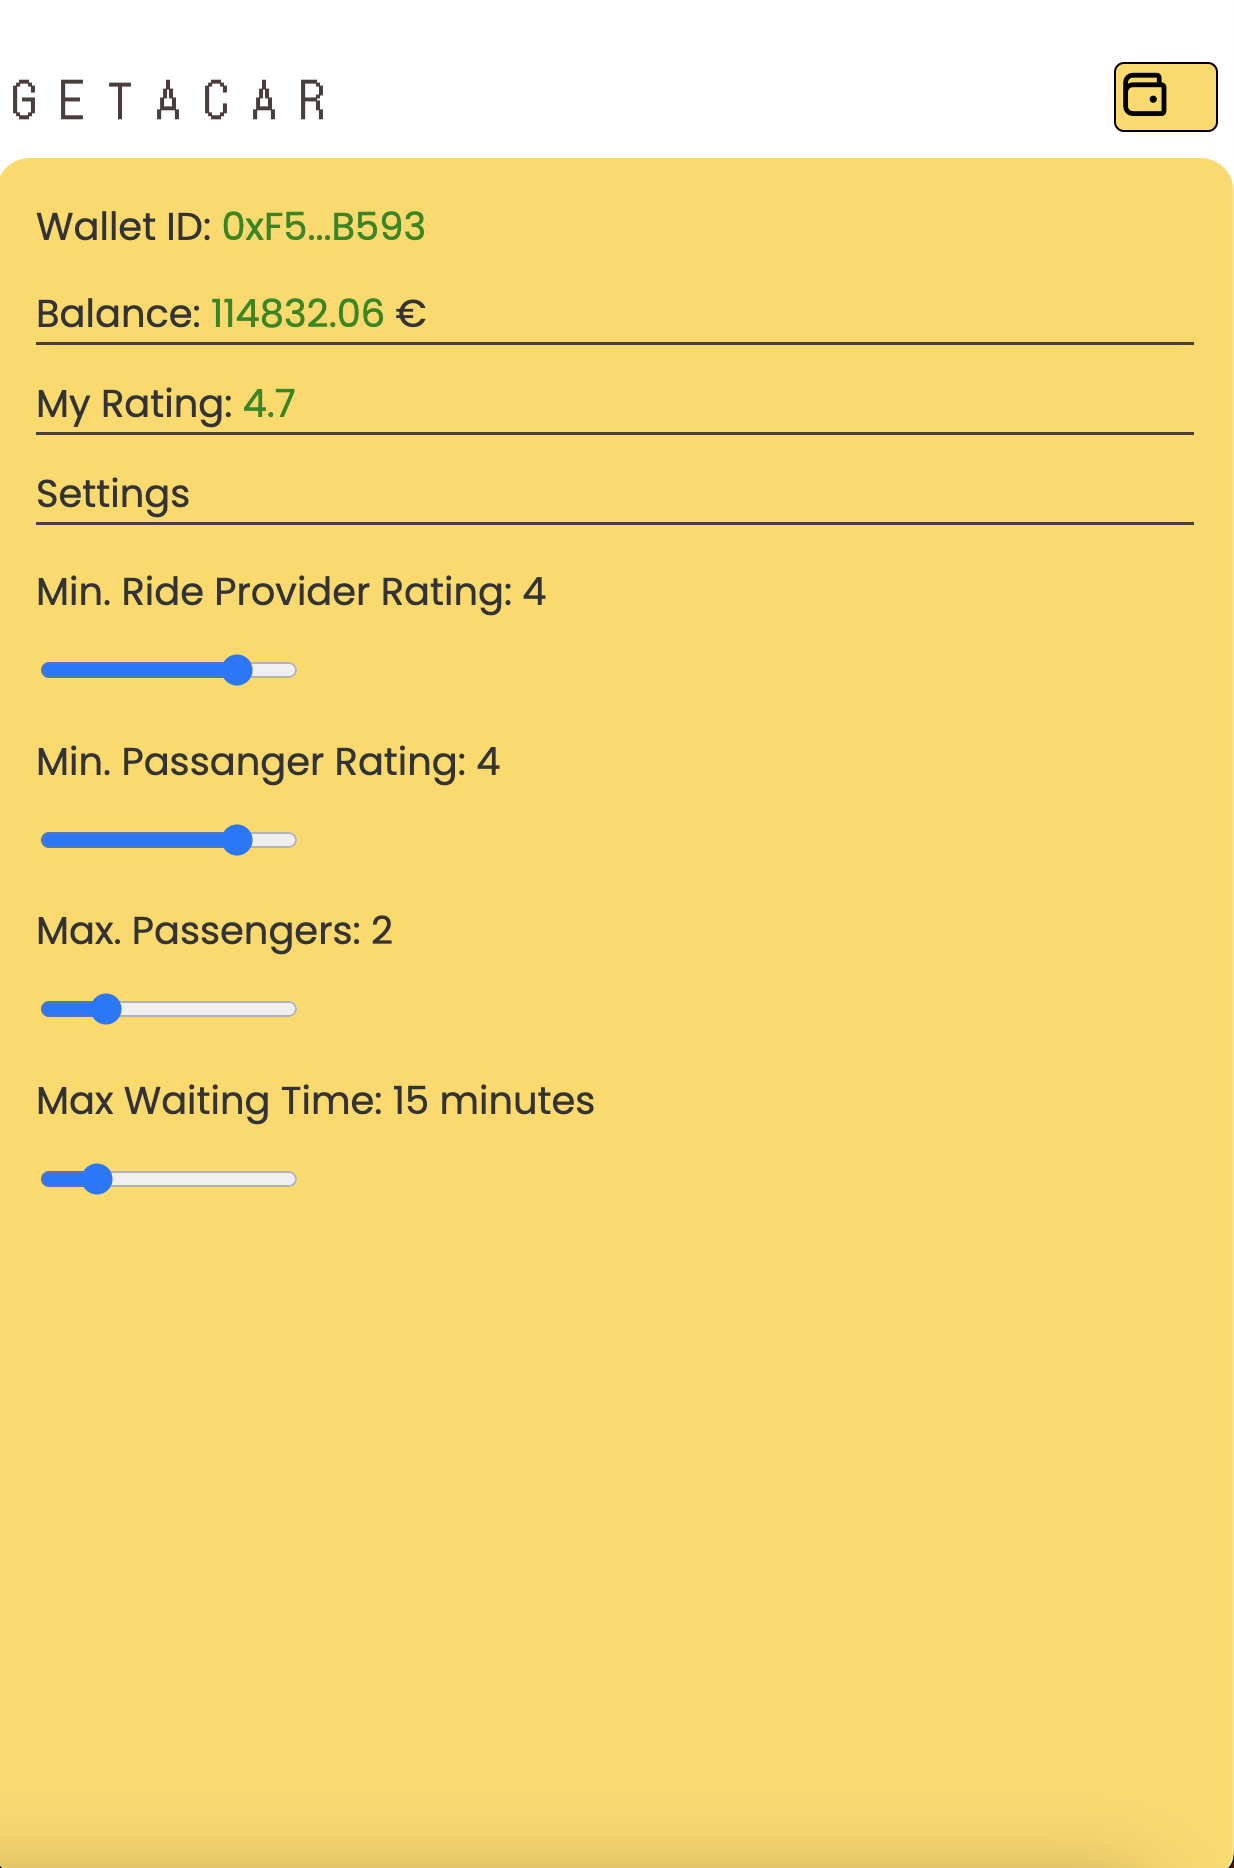
\includegraphics[width=0.45\linewidth]{data/ffss/13.png}
    \caption{Frontend: Settings Screen}
    \label{fig:SettingsScreen}
\end{figure}


\subsection{Customer Frontend Logic}
Now that the user flow of the customer frontend is shown, it is important to take a short look at the code logic behind the UI. While most of the logic behind the frontend is standard angular code, the utilisation of the web3\footnote{https://www.npmjs.com/package/web3} package is notable, as it allows the frontend to interact with smart contracts directly. To demonstrate this interaction, the \texttt{setUserReadyToStartRide()} function is chosen as an example. This function gets triggered when a customer presses the ''Start Driving'' button shown in \ref{fig:VehicleArrivedScreen}. First, the function checks if a wallet is connected with the frontend. The prototype utilises the external wallet provider MetaMask\footnote{https://metamask.io} to manage multiple wallets. After the check is successful, the function initiates a new, local instance of the contract. Once this is done successfully, the method calls the \texttt{setUserReadyToStartRide()} function inside the ride contract with an encrypted \texttt{userReadyToStartRideMessage} as input, first to calculate the excepted Gas fee and after the transaction is confirmed through Meta Mask by the user, a second time to actually trigger the \texttt{setUserReadyToStartRide()} function inside the ride contract, as seen in \ref{lst:setUserReadyToStartRide}.

\definecolor{verylightgray}{rgb}{.97,.97,.97}

% Define the JavaScript language for lstlisting
\lstdefinelanguage{JavaScript}{
  keywords={typeof, new, true, false, catch, function, return, null, catch, switch, var, if, in, while, do, else, case, break, async, await, const, let, on},
  keywordstyle=\color{blue}\bfseries,
  ndkeywords={class, export, boolean, throw, implements, import, this},
  ndkeywordstyle=\color{darkgray}\bfseries,
  identifierstyle=\color{black},
  sensitive=false,
  comment=[l]{//},
  morecomment=[s]{/*}{*/},
  commentstyle=\color{gray}\ttfamily,
  stringstyle=\color{red}\ttfamily,
  morestring=[b]',
  morestring=[b]"
}

\lstset{
	language=JavaScript, % <-- Change this to JavaScript
	backgroundcolor=\color{verylightgray},
	extendedchars=true,
	basicstyle=\footnotesize\ttfamily,
	showstringspaces=false,
	showspaces=false,
	numbers=left,
	numberstyle=\footnotesize,
	numbersep=9pt,
	tabsize=2,
	breaklines=true,
	showtabs=false,
	captionpos=b
}

\begin{Listing}
\begin{lstlisting}
  async setUserReadyToStartRide(){

    if (!this.web3) {
      console.error('Wallet not connected');
      return;
    }

    const accounts = await this.web3.eth.getAccounts();
    const selectedAddress = accounts[0];

    // Initialize the contract instance
    this.contract = new this.web3.eth.Contract(
      contractAbi as AbiItem[],
      this.rideContractAddress,
    );

    // Call the createContract function
    const gasEstimate = await this.contract.methods
      .setUserReadyToStartRide(userReadyToStartRideMessage)
      .estimateGas({ from: selectedAddress });

    this.contract.methods
      .setUserReadyToStartRide(userReadyToStartRideMessage)
      .send({ from: selectedAddress, gas: gasEstimate })
      .on('transactionHash', (hash: string) => {
        console.log('Transaction hash:', hash);
      })
      .on('receipt', (receipt: any) => {
        console.log('Transaction receipt events:', receipt);
      })

      .on('error', (error: Error) => {
        console.error('Error:', error);
      });
  }
\end{lstlisting}
  \caption{booking.component.ts:   async setUserReadyToStartRide() Function}
  \label{lst:setUserReadyToStartRide}
\end{Listing}

All functions that are contained within the customer frontend follow this basic flow to interact with the ride contract on the blockchain.


\subsection{Virtual Vehicle}
The Virtual Vehicle represents a new component introduced for the prototype implementation of the GETACAR platform. The Virtual Vehicle is a software daemon that automatically interacts with the platform as a ride provider. The Virtual Vehicle is written in Node.js and utilises the same web3 package implementation to interact with the blockchain as the customer frontend. It differentiates itself from the customer frontend by not providing a user frontend but by interacting with the platform in an automated way. When starting the Virtual Vehicle, it automatically connects to a predefined matching service and begins to scan for open ride requests. Once it has found a ride request it automatically bids a random amount of money to handle the right. If the Virtual Vehicle wins the auction, it will sign the ride contract and start to follow the predefined ride flow until the right is completed. Once the ride is completed or in case the Virtual Vehicle does not win the auction, it starts to bid on new ride requests. To test the platform and the matching service, it is possible to spin up multiple Virtual Vehicles that all simultaneously interact with the platform. 
In conclusion, the Virtual Vehicles help with simulating platform traffic and testing the prototypical implementation of the GETACAR platform by acting as virtual ride providers. 